\documentclass{beamer}
\usetheme{Boadilla}
\usecolortheme{dolphin}
\usefonttheme{serif}
\setbeamertemplate{navigation symbols}{}
\setbeamertemplate{caption}[numbered]
\usepackage{graphicx}
\usepackage{amsmath}
\usepackage{hyperref}
\usepackage{booktabs}
\usepackage{multicol}
\usepackage{pgfplots}
\pgfplotsset{compat=1.18}

\title{An Economic Analysis of Optimal Investment Strategies for Accumulating Housing Down Payments}
\author{Frank Paul Longo II}
\date{\today}

\begin{document}

\begin{frame}
    \titlepage
\end{frame}

\section{Introduction}
\begin{frame}{Introduction}
    \begin{block}{Objective}
        Develop optimal investment strategies for first-time homebuyers to save for down payments.
    \end{block}
    \begin{block}{Research Question}
        What are the optimal investment strategies for aspiring first-time homebuyers of various age cohorts to accumulate down payments over 5, 10, and 15-year investment horizons?
    \end{block}
    \begin{block}{Motivation}
        Address the challenges posed by escalating housing costs and assist diverse age groups in expediting their path to homeownership.
    \end{block}
\end{frame}

\section{Financial Literacy: Essential Concepts}
\begin{frame}{Essential Financial Concepts}
    \begin{block}{Stocks}
        Equity investments representing proprietorship in a company.
    \end{block}
    \begin{block}{Mutual Funds}
        Investment vehicles that aggregate capital from numerous investors to purchase a diversified portfolio of stocks, bonds, or other securities.
    \end{block}
    \begin{block}{ETFs (Exchange-Traded Funds)}
        Analogous to mutual funds but traded on stock exchanges like individual stocks.
    \end{block}
\end{frame}

\section{Typical First-time Homebuyer Profile}
\begin{frame}{Typical First-time Homebuyer Profile}
    \begin{block}{Demographics}
        \begin{itemize}
            \item \textbf{Median Age:} 35 years (2024)\footnote{National Association of Realtors, 2024 Profile of Home Buyers and Sellers.}
            \item \textbf{Median Household Income:} \$104,000 (2024)\footnote{Consumer Financial Protection Bureau, Market Snapshot: First-time Homebuyers, 2024.}
            \item \textbf{Median Nationwide Home Cost:} \$416,100 (2024)\footnote{U.S. Department of Housing and Urban Development, 2024.}
        \end{itemize}
    \end{block}
\end{frame}

\section{Risk Tolerances and Investment Contributions}
\begin{frame}{Investment Contributions by Age Group}
    \begin{block}{20-25 Years Old (15-Year Time Horizon)}
        \begin{itemize}
            \item \textbf{Median Gross Income:} \$45,000\footnote{Bureau of Labor Statistics, 2024.}
            \item \textbf{Annual Contribution:} 10\%\footnote{Federal Reserve, 2024.}
            \item \textbf{Risk Tolerance (Beta):} 1.2\footnote{Morgan Stanley, 2024.}
            \item \textbf{Equity Breakdown:}
            \begin{itemize}
                \item Stocks: 50\%\footnote{Empower, 2024.}
                \item Mutual Funds: 25\%\footnote{Charles Schwab, 2024.}
                \item ETFs: 25\%\footnote{J.P. Morgan, 2024.}
            \end{itemize}
        \end{itemize}
    \end{block}
\end{frame}

\begin{frame}{Investment Contributions by Age Group}
    \begin{block}{25-30 Years Old (10-Year Time Horizon)}
        \begin{itemize}
            \item \textbf{Median Gross Income:} \$60,000\footnote{Bureau of Labor Statistics, 2024.}
            \item \textbf{Annual Contribution:} 15\%\footnote{Federal Reserve, 2024.}
            \item \textbf{Risk Tolerance (Beta):} 1.0\footnote{Morgan Stanley, 2024.}
            \item \textbf{Equity Breakdown:}
            \begin{itemize}
                \item Stocks: 45\%\footnote{Morgan Stanley, 2024.}
                \item Mutual Funds: 30\%\footnote{Charles Schwab, 2024.}
                \item ETFs: 25\%\footnote{J.P. Morgan, 2024.}
            \end{itemize}
        \end{itemize}
    \end{block}
\end{frame}

\begin{frame}{Investment Contributions by Age Group}
    \begin{block}{30-35 Years Old (5-Year Time Horizon)}
        \begin{itemize}
            \item \textbf{Median Gross Income:} \$80,000\footnote{Bureau of Labor Statistics, 2024.}
            \item \textbf{Annual Contribution:} 20\%\footnote{Federal Reserve, 2024.}
            \item \textbf{Risk Tolerance (Beta):} 0.8\footnote{Morgan Stanley, 2024.}
            \item \textbf{Equity Breakdown:}
            \begin{itemize}
                \item Stocks: 40\%\footnote{Empower, 2024.}
                \item Mutual Funds: 35\%\footnote{Charles Schwab, 2024.}
                \item ETFs: 25\%\footnote{J.P. Morgan, 2024.}
            \end{itemize}
        \end{itemize}
    \end{block}
\end{frame}

\section{Data Import}
\begin{frame}{Data Sources}
    \begin{block}{Primary Source}
        \textbf{Yahoo Finance (YFinance)}
        \begin{itemize}
            \item Comprehensive financial data on stocks, mutual funds, and ETFs.
        \end{itemize}
    \end{block}

    \begin{block}{Data Coverage}
        \textbf{Date Range:} 10/24/2012 to present (daily frequency)
    \end{block}

    \begin{block}{Data Fields}
        \begin{multicols}{2}
        \begin{itemize}
            \item Open
            \item High
            \item Low
            \item Close
            \item Adj Close
            \item Volume
            \item Type
        \end{itemize}
        \end{multicols}
    \end{block}
\end{frame}

\section{Exploratory Data Analysis}
\begin{frame}[fragile]{Visualizing Security Count}
    \begin{figure}
        \centering
        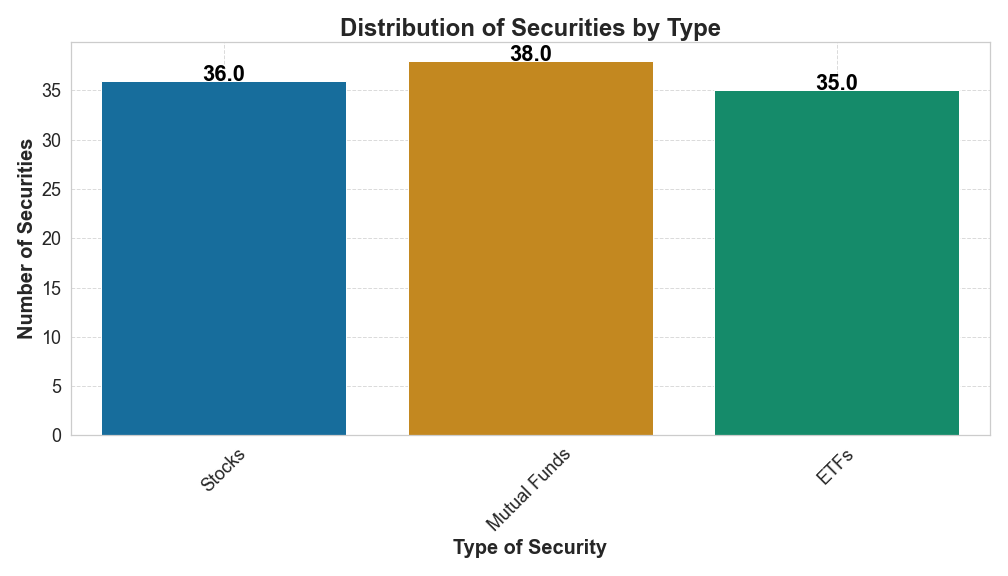
\includegraphics[width=\textwidth]{histogram_security_count.png}
    \end{figure}
\end{frame}

\begin{frame}[fragile]{Visualizing Returns Distribution}
        \begin{figure}
            \centering
            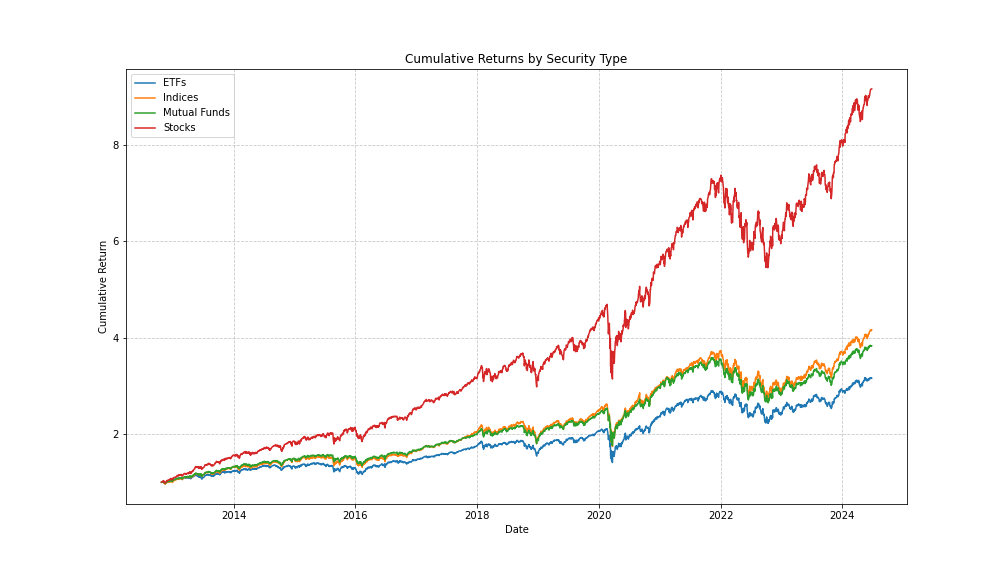
\includegraphics[width=\textwidth]{cumulative_returns_by_type.png}
        \end{figure}
\end{frame}

\section{CAPM}
\begin{frame}{Capital Asset Pricing Model (CAPM)}
    \begin{block}{Formula} 
        \begin{equation*}
            E(R_i) = R_f + \beta_i (E(R_m) - R_f)
        \end{equation*}
        \footnote{Sharpe, W. F. (1964). Capital asset prices: A theory of market equilibrium under conditions of risk. \textit{The Journal of Finance}, 19(3), 425-442.}
    \end{block}
    \begin{block}{Assumptions}
        \begin{itemize}
            \item Diversified portfolios
            \item Efficient markets
            \item No taxes or transaction costs
            \item Constant risk-free rate
        \end{itemize}
    \end{block}
\end{frame}

\begin{frame}[fragile]{Calculating Beta}
    \begin{block}{Market Return Calculation}
        \begin{verbatim}
# Market return (e.g., S&P 500)
market = yf.download('^GSPC', start='2012-10-24', end='2024-09-26')
market_returns = market['Adj Close'].pct_change().dropna()

# Calculate beta for each stock
beta = {}
for ticker in tickers:
    cov_matrix = np.cov(returns[ticker], market_returns)
    beta[ticker] = cov_matrix[0, 1] / cov_matrix[1, 1]
        \end{verbatim}
    \end{block}
\end{frame}

\begin{frame}[fragile]{Calculating Expected Return using CAPM}
    \begin{block}{Expected Return Calculation}
        \begin{verbatim}
# Assuming a risk-free rate of 3% and market return of 8%
risk_free_rate = 0.03
market_return = 0.08

# Calculate expected return for each stock
capm_returns = {}
for ticker in tickers:
    capm_returns[ticker] = risk_free_rate + beta[ticker] * 
    (market_return - risk-free_rate)
        \end{verbatim}
    \end{block}
\end{frame}

\begin{frame}{Actual Return vs. CAPM Expected Return (5 Year Time Horizon)}
    \centering
    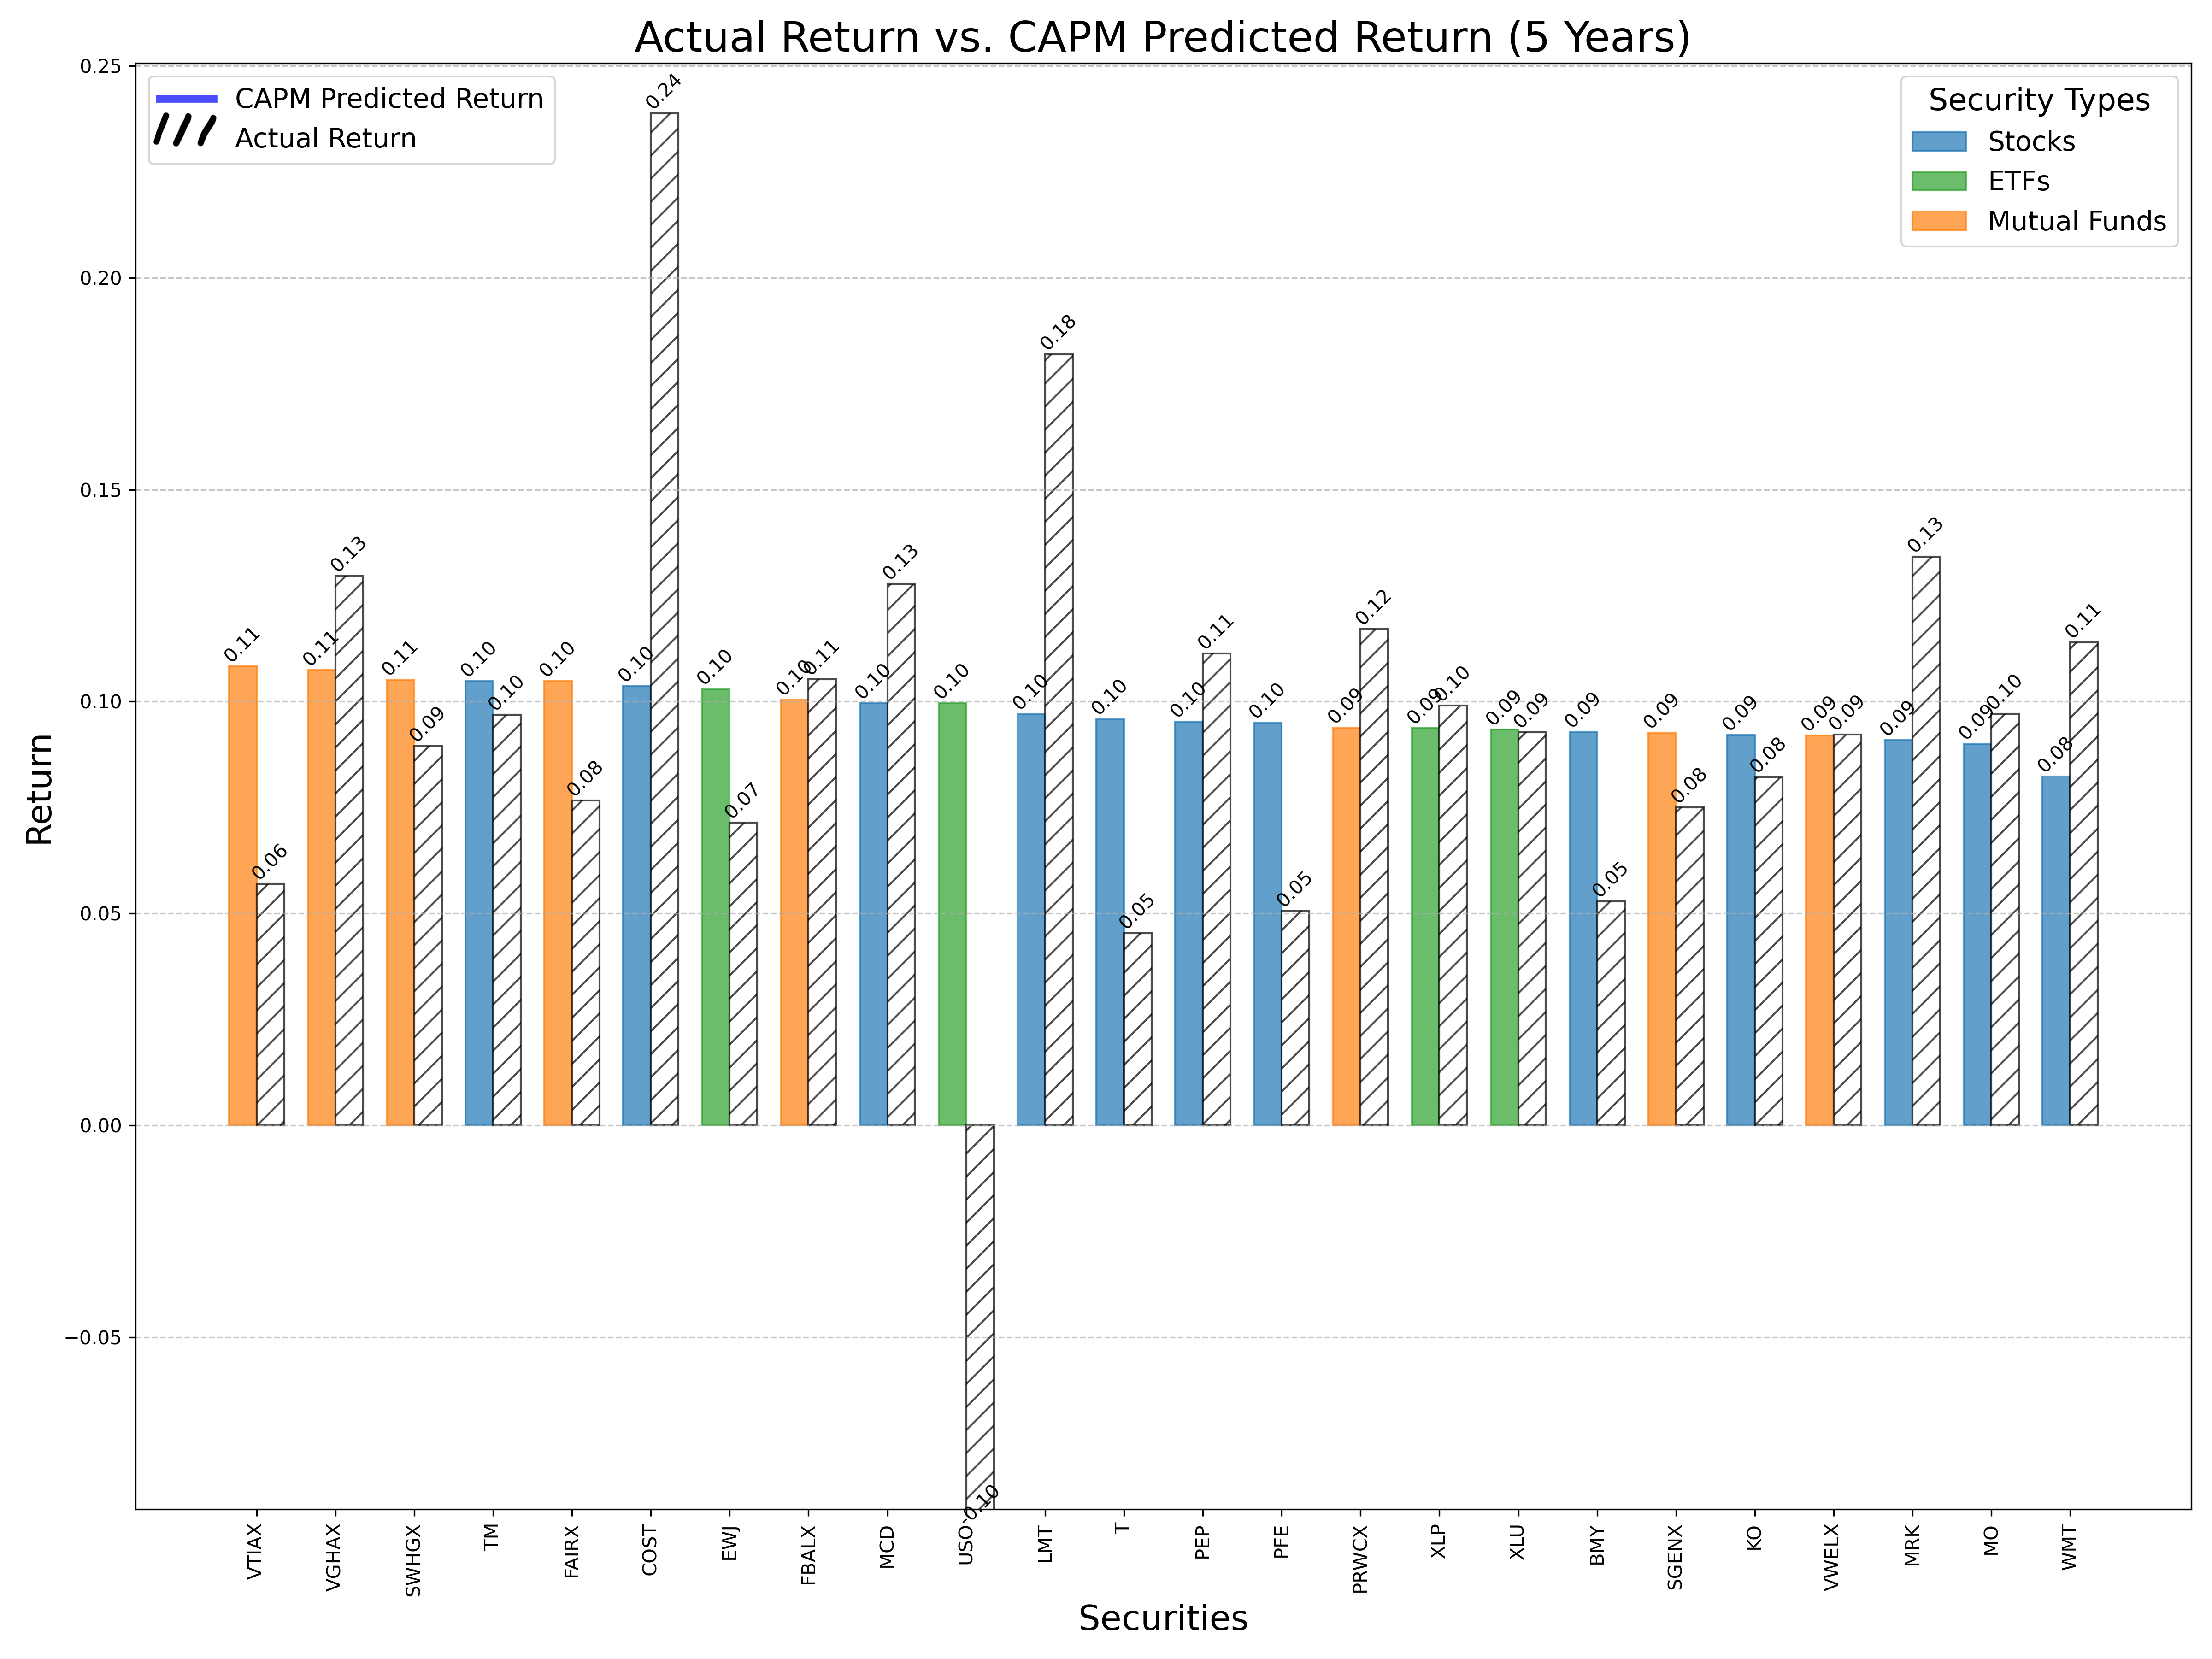
\includegraphics[height=0.8\textheight]{actual_vs_capm_5_years.png}
\end{frame}

\begin{frame}{Actual Return vs. CAPM Expected Return (10 Year Time Horizon)}
    \centering
    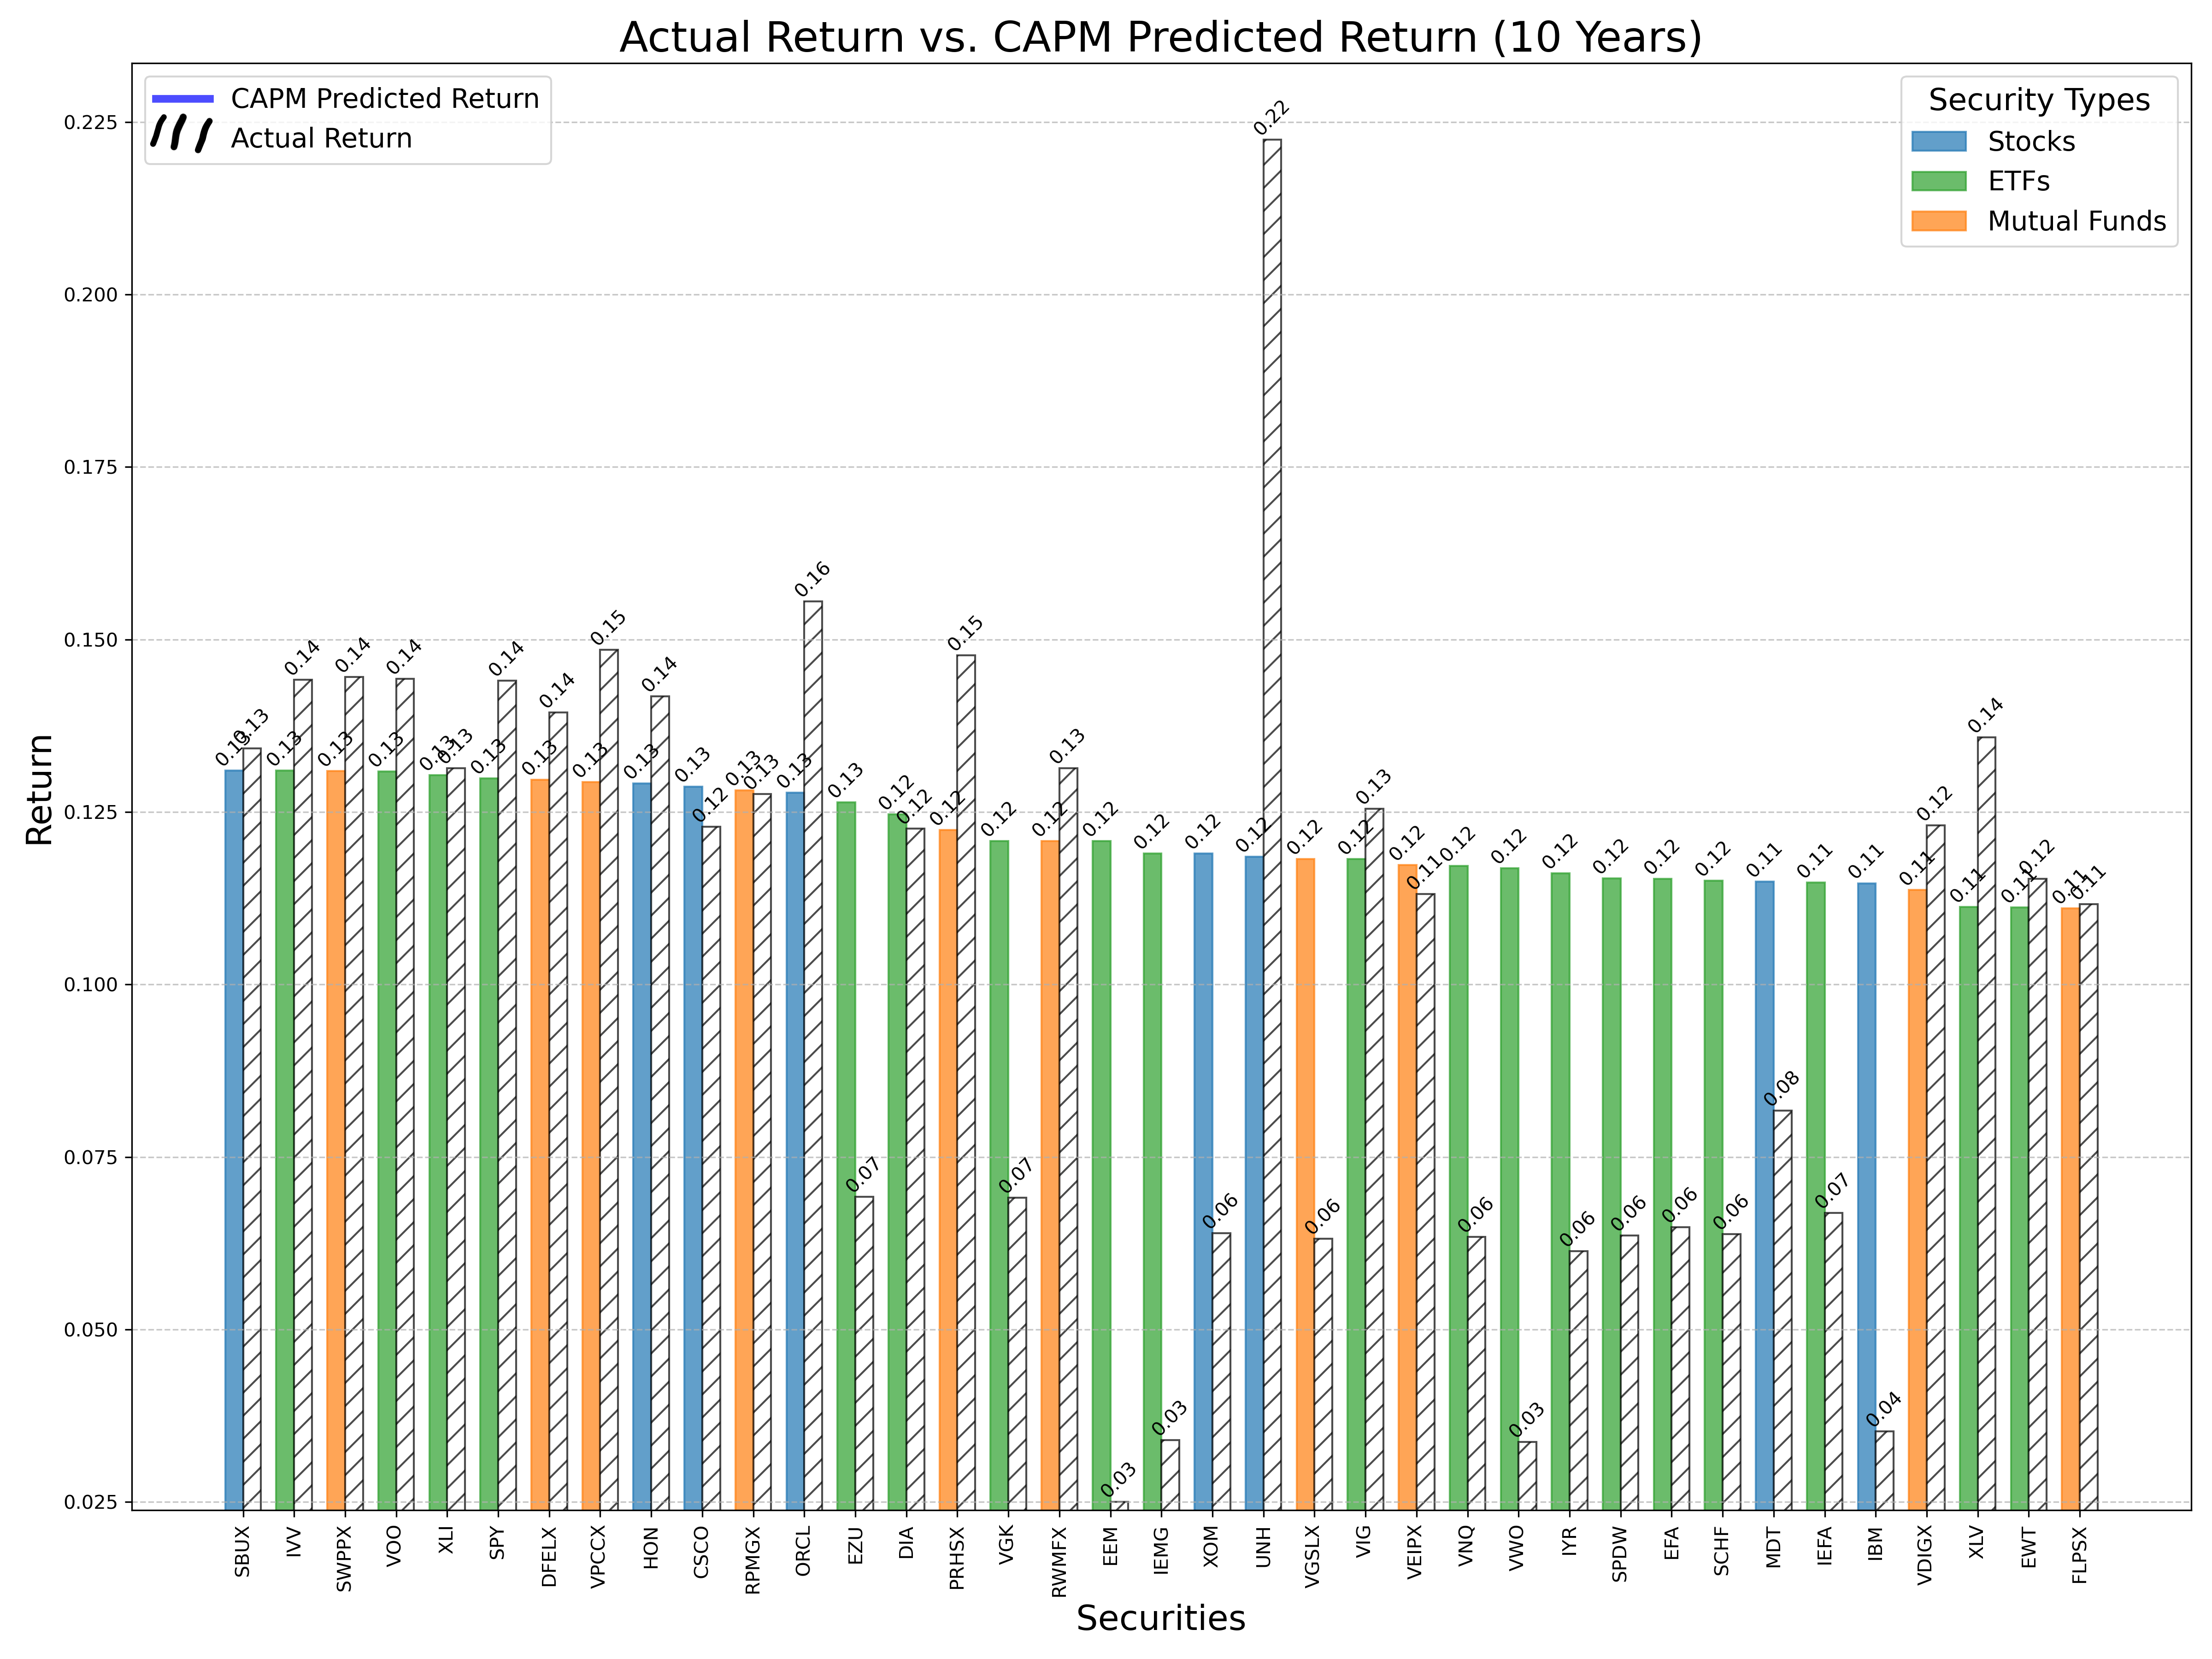
\includegraphics[height=0.8\textheight]{actual_vs_capm_10_years.png}
\end{frame}

\begin{frame}{Actual Return vs. CAPM Expected Return (15 Year Time Horizon)}
    \centering
    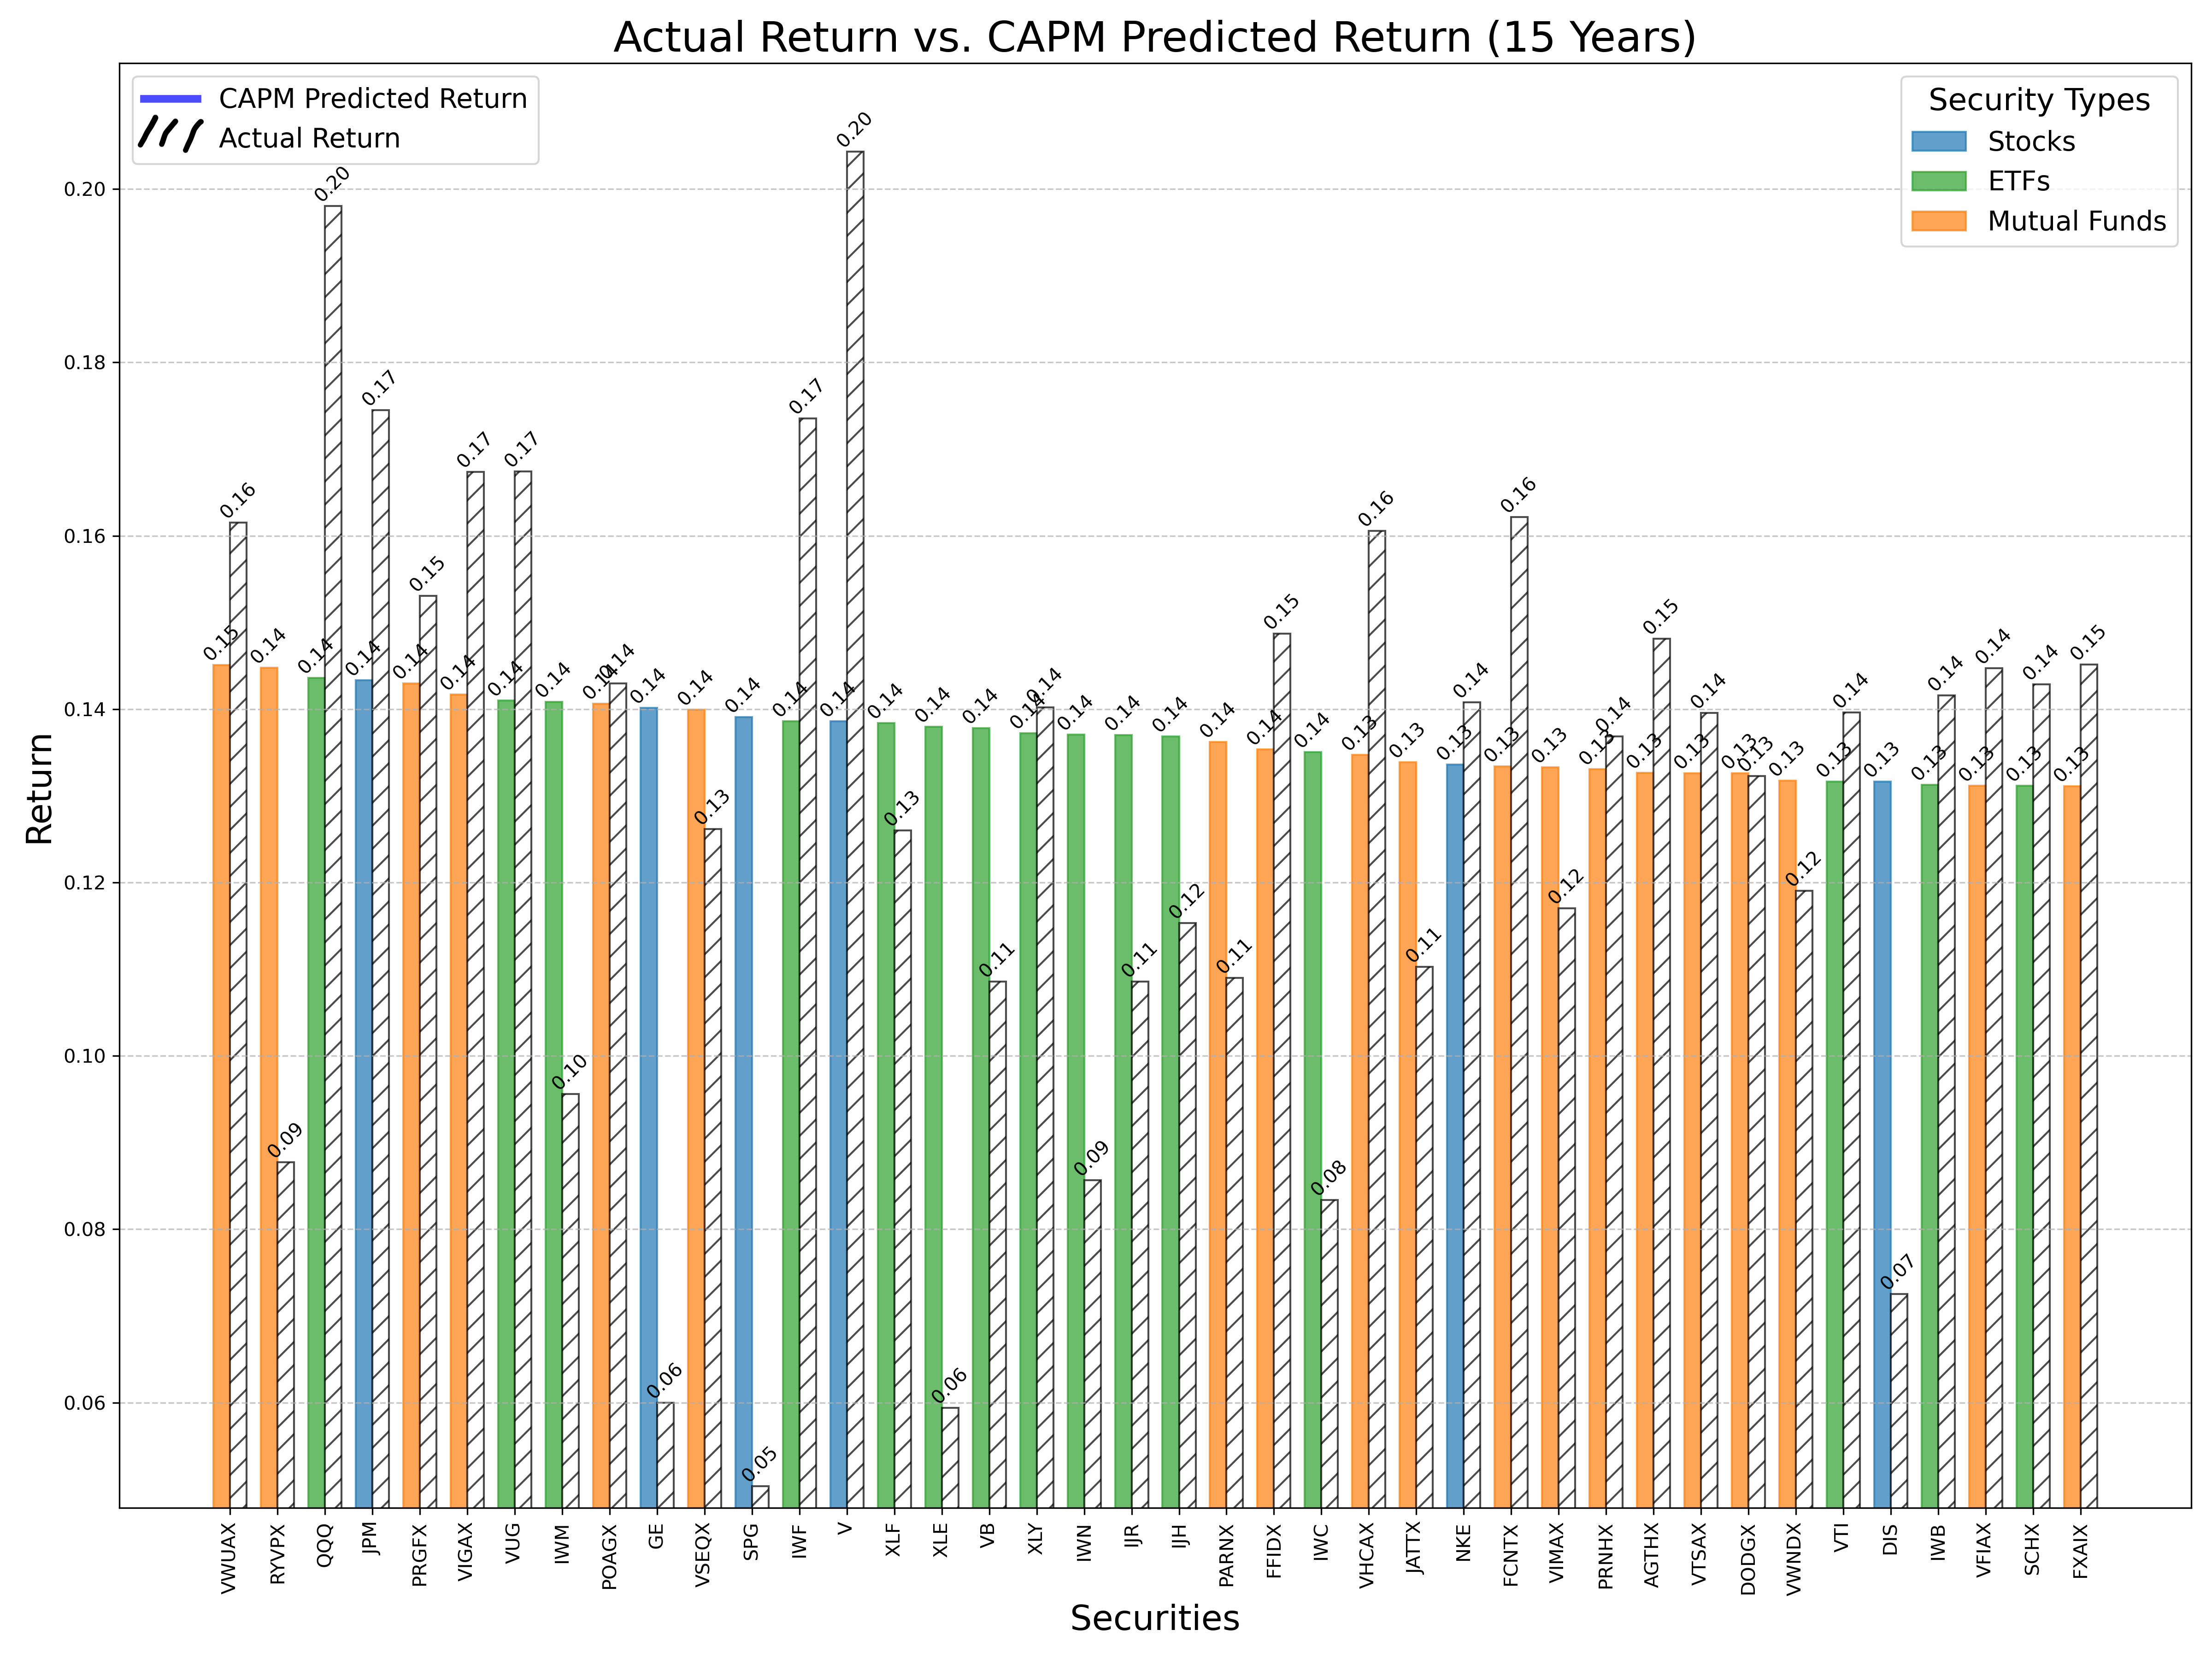
\includegraphics[height=0.8\textheight]{actual_vs_capm_15_years.png}
\end{frame}

\section{New Filtered Data}
\begin{frame}{Resulting Filtered Data Generated (For Each Time Horizon)}
    \begin{block}{Data Fields}
        \begin{multicols}{2}
        \begin{itemize}
            \item Ticker
            \item Beta
            \item CAPM
            \item Predicted Return
            \item Actual Return
            \item Volatility
            \item Sharpe Ratio
            \item Type
        \end{itemize}
        \end{multicols}
    \end{block}
\end{frame}

\section{Modern Portfolio Theory (MPT)}
\begin{frame}{Modern Portfolio Theory (MPT)}
    \begin{block}{Overview}
        A framework for constructing a portfolio to maximize return for a given level of risk.\footnote{Markowitz, H. (1952). Portfolio Selection. \textit{The Journal of Finance}, 7(1), 77-91.}
    \end{block}
    \begin{block}{Formulas}
            \begin{equation*}
                \sigma_p^2 = \sum_{i=1}^{n} \sum_{j=1}^{n} w_i w_j \sigma_{ij}
            \end{equation*}
    \end{block}
    \begin{block}{Definitions}
        \begin{multicols}{2}
            \begin{itemize}
                \item \(E(R_p)\): Portfolio return
                \item \(w_i\): Weight of asset \(i\)
                \item \(E(R_i)\): Return of asset \(i\)
                \item \(\sigma_p^2\): Portfolio variance
                \item \(\sigma_{ij}\): Covariance of assets \(i, j\)
            \end{itemize}
        \end{multicols}
    \end{block}
\end{frame}

\section{Portfolio Optimization}
\begin{frame}{Optimize the Portfolio}
    \begin{block}{Objective}
        Adjust the weights of the assets to maximize the portfolio's expected return for a given level of risk or to minimize risk for a given level of expected return.
    \end{block}
    \begin{block}{Optimization Problem}
        Solve the following optimization problem:
        \begin{equation*}
            \min \sigma_p^2 = \sum_{i=1}^{n} \sum_{j=1}^{n} w_i w_j \sigma_{ij}
        \end{equation*}
        Subject to:
        \begin{equation*}
            \sum_{i=1}^{n} w_i = 1 \quad \text{and} \quad E(R_p) = \sum_{i=1}^{n} w_i E(R_i)
        \end{equation*}
    \end{block}
\end{frame}


\begin{frame}[fragile]{Setting Up the Optimization}
    \begin{block}{Bounds and Optimization Process}
        \scriptsize
        \begin{verbatim}
# Bounds to ensure diversification
bounds = tuple((0.0, 0.1) for _ in range(num_assets))

# Optimize the portfolio
result = minimize(negative_sharpe_ratio, init_guess, 
                  args=(mean_returns, cov_matrix, risk_free_rate), 
                  method='SLSQP', bounds=bounds, constraints=constraints)
        \end{verbatim}
    \end{block}
    \begin{block}{Explanation}
        \scriptsize
        \begin{itemize}
            \item \textbf{Bounds}: Limit the weight of any single asset to a maximum of 10% to ensure diversification.
            \item \textbf{Optimization}: Use the SLSQP method to find the optimal weights that maximize the Sharpe ratio by minimizing its negative.
        \end{itemize}
    \end{block}
\end{frame}

\begin{frame}{Optimal Portfolio (5 Years)}
    \centering
    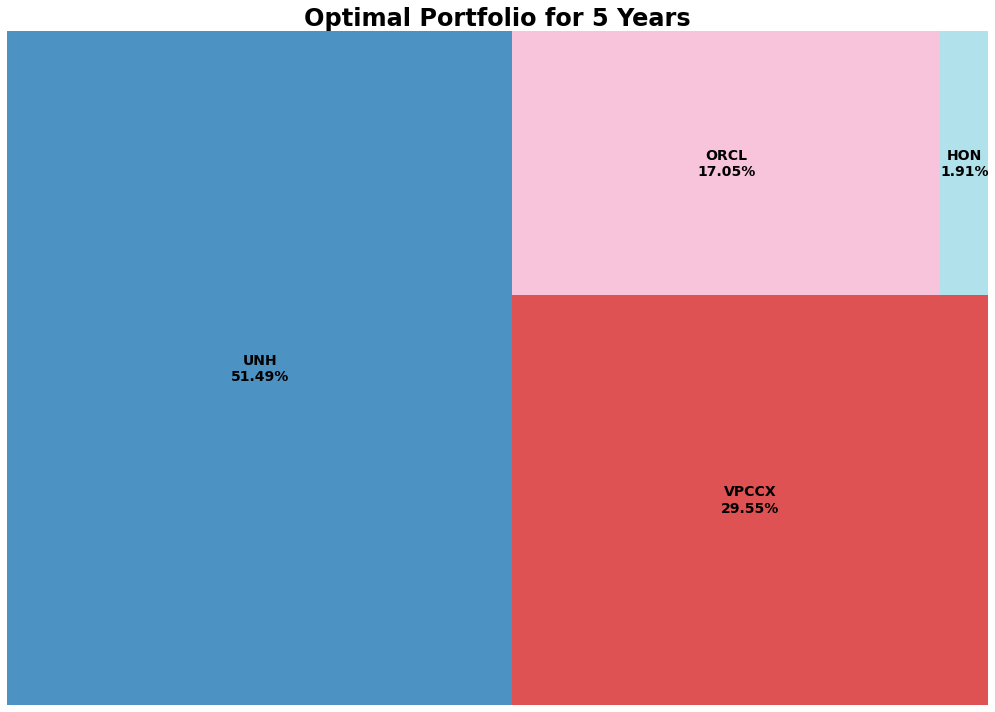
\includegraphics[height=0.8\textheight]{optimal_portfolio_5_years.png}
\end{frame}

\begin{frame}{Optimal Portfolio (10 Years)}
    \centering
    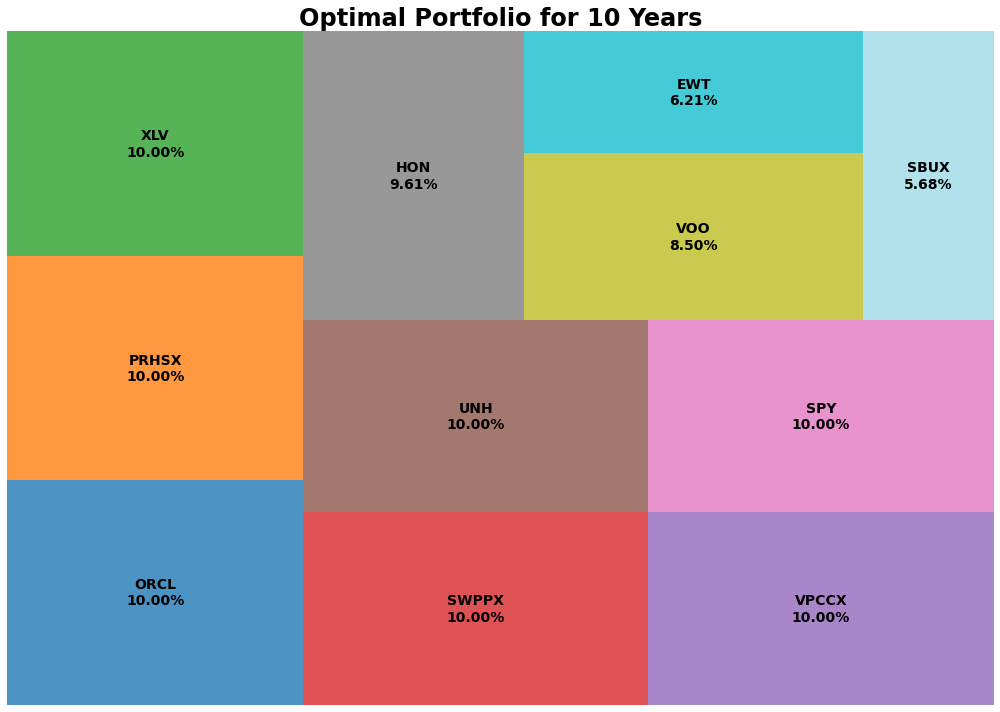
\includegraphics[height=0.8\textheight]{optimal_portfolio_10_years.png}
\end{frame}

\begin{frame}{Optimal Portfolio (15 Years)}
    \centering
    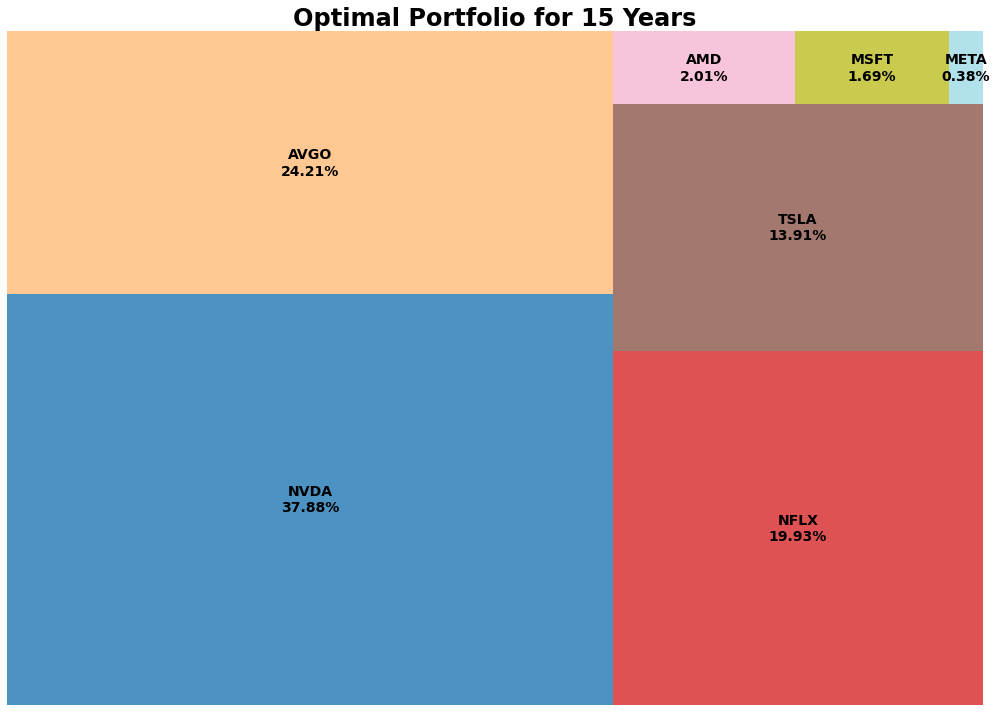
\includegraphics[height=0.8\textheight]{optimal_portfolio_15_years.png}
\end{frame}

\section{Results Interpretation}
\begin{frame}{Results Interpretation}
    \begin{block}{Findings}
        Through this analysis using the Capital Asset Pricing Model (CAPM) and Modern Portfolio Theory (MPT), we successfully identified the optimal weights for the selected securities. The analysis revealed that diversification across different asset classes and strategic allocation can significantly enhance the potential for accumulating sufficient down payments over varying time horizons.
    \end{block}
    \begin{block}{Implications}
        These findings underscore the importance of tailored investment strategies for different age groups and income levels. By leveraging these models, first-time homebuyers can make informed decisions that align with their financial goals and risk tolerance.
    \end{block}
\end{frame}

\section{Future Work and Limitations}
\begin{frame}{Future Work and Limitations}
    \begin{block}{Future Work}
        In future research, I plan to incorporate Monte Carlo Simulations to forecast future trends for the optimized portfolio. This will provide a more robust understanding of potential investment outcomes under various market conditions.
    \end{block}
    \begin{block}{Limitations}
        This study's limitations include the assumption of constant risk-free rates and market returns, as well as the exclusion of transaction costs and taxes. Future work should aim to address these limitations to enhance the model's accuracy and applicability.
    \end{block}
\end{frame}

\begin{frame}{Q\&A}
    \begin{block}{Questions and Clarifications}
        Please feel free to ask for any clarifications or additional details regarding the presented research and findings.
    \end{block}
    \vspace{1cm}
    \begin{center}
        \Large \textbf{Thank you for your attention!}
    \end{center}
\end{frame}

\begin{frame}{References (1/2)}
    \begin{block}{}
        \begin{itemize}
            \item Boyle, P. P. (1977). Options: A Monte Carlo Approach. \textit{Journal of Financial Economics, 4}(3), 323-338. DOI: 10.1016/0304-405X(77)90005-8
            \item Federal Reserve. (2023). Report on the Economic Well-Being of U.S. Households in 2023. Retrieved from \url{https://www.federalreserve.gov/publications/2023-economic-well-being-of-us-households-in-2023.htm}
            \item Investment Company Institute. (n.d.). Retrieved from \url{https://www.ici.org/}
            \item Markowitz, H. (1952). Portfolio Selection. \textit{Journal of Finance, 7}(1), 77-91. DOI: 10.2307/2975974
        \end{itemize}
    \end{block}
\end{frame}

\begin{frame}{References (2/2)}
    \begin{block}{}
        \begin{itemize}
            \item Morgan Stanley. (2024). Risk Tolerance Report. Retrieved from \url{https://www.morganstanley.com/}
            \item National Association of Realtors. (2023). 2023 Home Buyer and Seller Generational Trends. Retrieved from \url{https://www.nar.realtor/research-and-statistics/research-reports/home-buyer-and-seller-generational-trends}
            \item Sharpe, W. F. (1964). Capital Asset Prices: A Theory of Market Equilibrium under Conditions of Risk. \textit{The Journal of Finance, 19}(3), 425-442. DOI: 10.2307/2975974
            \item Sharpe, W. F. (1966). Mutual Fund Performance. \textit{Journal of Business, 39}(1), 119-138. DOI: 10.1086/294846
            \item U.S. Department of Housing and Urban Development. (2024). Housing Market Analysis. Retrieved from \url{https://www.hud.gov/}
            \item Yahoo Finance. (n.d.). Retrieved from \url{https://finance.yahoo.com/}
        \end{itemize}
    \end{block}
\end{frame}

\end{document}
